\documentclass[twoside]{book}

% Packages required by doxygen
\usepackage{calc}
\usepackage{doxygen}
\usepackage{graphicx}
\usepackage[utf8]{inputenc}
\usepackage{makeidx}
\usepackage{multicol}
\usepackage{multirow}
\usepackage{fixltx2e}
\PassOptionsToPackage{warn}{textcomp}
\usepackage{textcomp}
\usepackage[nointegrals]{wasysym}
\usepackage[table]{xcolor}

% Font selection
\usepackage[T1]{fontenc}
\usepackage{mathptmx}
\usepackage[scaled=.90]{helvet}
\usepackage{courier}
\usepackage{amssymb}
\usepackage{sectsty}
\renewcommand{\familydefault}{\sfdefault}
\allsectionsfont{%
  \fontseries{bc}\selectfont%
  \color{darkgray}%
}
\renewcommand{\DoxyLabelFont}{%
  \fontseries{bc}\selectfont%
  \color{darkgray}%
}
\newcommand{\+}{\discretionary{\mbox{\scriptsize$\hookleftarrow$}}{}{}}

% Page & text layout
\usepackage{geometry}
\geometry{%
  a4paper,%
  top=2.5cm,%
  bottom=2.5cm,%
  left=2.5cm,%
  right=2.5cm%
}
\tolerance=750
\hfuzz=15pt
\hbadness=750
\setlength{\emergencystretch}{15pt}
\setlength{\parindent}{0cm}
\setlength{\parskip}{0.2cm}
\makeatletter
\renewcommand{\paragraph}{%
  \@startsection{paragraph}{4}{0ex}{-1.0ex}{1.0ex}{%
    \normalfont\normalsize\bfseries\SS@parafont%
  }%
}
\renewcommand{\subparagraph}{%
  \@startsection{subparagraph}{5}{0ex}{-1.0ex}{1.0ex}{%
    \normalfont\normalsize\bfseries\SS@subparafont%
  }%
}
\makeatother

% Headers & footers
\usepackage{fancyhdr}
\pagestyle{fancyplain}
\fancyhead[LE]{\fancyplain{}{\bfseries\thepage}}
\fancyhead[CE]{\fancyplain{}{}}
\fancyhead[RE]{\fancyplain{}{\bfseries\leftmark}}
\fancyhead[LO]{\fancyplain{}{\bfseries\rightmark}}
\fancyhead[CO]{\fancyplain{}{}}
\fancyhead[RO]{\fancyplain{}{\bfseries\thepage}}
\fancyfoot[LE]{\fancyplain{}{}}
\fancyfoot[CE]{\fancyplain{}{}}
\fancyfoot[RE]{\fancyplain{}{\bfseries\scriptsize Generated on Tue Jul 22 2014 07\+:58\+:01 for A\+Y\+D\+P Base Station by Doxygen }}
\fancyfoot[LO]{\fancyplain{}{\bfseries\scriptsize Generated on Tue Jul 22 2014 07\+:58\+:01 for A\+Y\+D\+P Base Station by Doxygen }}
\fancyfoot[CO]{\fancyplain{}{}}
\fancyfoot[RO]{\fancyplain{}{}}
\renewcommand{\footrulewidth}{0.4pt}
\renewcommand{\chaptermark}[1]{%
  \markboth{#1}{}%
}
\renewcommand{\sectionmark}[1]{%
  \markright{\thesection\ #1}%
}

% Indices & bibliography
\usepackage{natbib}
\usepackage[titles]{tocloft}
\setcounter{tocdepth}{3}
\setcounter{secnumdepth}{5}
\makeindex

% Hyperlinks (required, but should be loaded last)
\usepackage{ifpdf}
\ifpdf
  \usepackage[pdftex,pagebackref=true]{hyperref}
\else
  \usepackage[ps2pdf,pagebackref=true]{hyperref}
\fi
\hypersetup{%
  colorlinks=true,%
  linkcolor=blue,%
  citecolor=blue,%
  unicode%
}

% Custom commands
\newcommand{\clearemptydoublepage}{%
  \newpage{\pagestyle{empty}\cleardoublepage}%
}


%===== C O N T E N T S =====

\begin{document}

% Titlepage & ToC
\hypersetup{pageanchor=false,
             bookmarks=true,
             bookmarksnumbered=true,
             pdfencoding=unicode
            }
\pagenumbering{roman}
\begin{titlepage}
\vspace*{7cm}
\begin{center}%
{\Large A\+Y\+D\+P Base Station \\[1ex]\large pre-\/1.\+0-\/0 }\\
\vspace*{1cm}
{\large Generated by Doxygen 1.8.7}\\
\vspace*{0.5cm}
{\small Tue Jul 22 2014 07:58:01}\\
\end{center}
\end{titlepage}
\clearemptydoublepage
\tableofcontents
\clearemptydoublepage
\pagenumbering{arabic}
\hypersetup{pageanchor=true}

%--- Begin generated contents ---
\chapter{Hierarchical Index}
\section{Class Hierarchy}
This inheritance list is sorted roughly, but not completely, alphabetically\+:\begin{DoxyCompactList}
\item Q\+Main\+Window\begin{DoxyCompactList}
\item \contentsline{section}{main\+Window}{\pageref{classmainWindow}}{}
\end{DoxyCompactList}
\item Q\+Widget\begin{DoxyCompactList}
\item \contentsline{section}{wind\+Data}{\pageref{classwindData}}{}
\end{DoxyCompactList}
\end{DoxyCompactList}

\chapter{Class Index}
\section{Class List}
Here are the classes, structs, unions and interfaces with brief descriptions\+:\begin{DoxyCompactList}
\item\contentsline{section}{\hyperlink{classmainWindow}{main\+Window} }{\pageref{classmainWindow}}{}
\item\contentsline{section}{\hyperlink{classwindData}{wind\+Data} }{\pageref{classwindData}}{}
\end{DoxyCompactList}

\chapter{File Index}
\section{File List}
Here is a list of all files with brief descriptions\+:\begin{DoxyCompactList}
\item\contentsline{section}{\hyperlink{sample_network_8cpp}{sample\+Network.\+cpp} }{\pageref{sample_network_8cpp}}{}
\item\contentsline{section}{\hyperlink{sample_network_8h}{sample\+Network.\+h} }{\pageref{sample_network_8h}}{}
\item\contentsline{section}{\hyperlink{sample_settings_8cpp}{sample\+Settings.\+cpp} }{\pageref{sample_settings_8cpp}}{}
\item\contentsline{section}{\hyperlink{sample_settings_8h}{sample\+Settings.\+h} }{\pageref{sample_settings_8h}}{}
\item\contentsline{section}{\hyperlink{wind_data_8cpp}{wind\+Data.\+cpp} }{\pageref{wind_data_8cpp}}{}
\item\contentsline{section}{\hyperlink{wind_data_8h}{wind\+Data.\+h} }{\pageref{wind_data_8h}}{}
\end{DoxyCompactList}

\chapter{Class Documentation}
\hypertarget{classmainWindow}{\section{main\+Window Class Reference}
\label{classmainWindow}\index{main\+Window@{main\+Window}}
}


{\ttfamily \#include $<$main\+Window.\+h$>$}



Inheritance diagram for main\+Window\+:\nopagebreak
\begin{figure}[H]
\begin{center}
\leavevmode
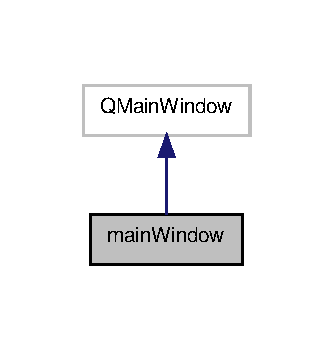
\includegraphics[width=160pt]{classmainWindow__inherit__graph}
\end{center}
\end{figure}


Collaboration diagram for main\+Window\+:\nopagebreak
\begin{figure}[H]
\begin{center}
\leavevmode
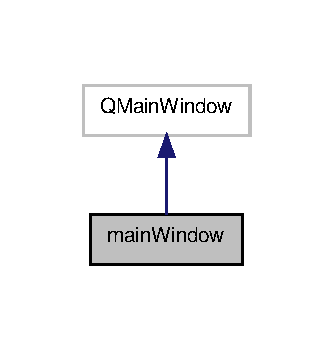
\includegraphics[width=160pt]{classmainWindow__coll__graph}
\end{center}
\end{figure}
\subsection*{Public Member Functions}
\begin{DoxyCompactItemize}
\item 
\hyperlink{classmainWindow_a4b70f914e07549dc4528c590af7cc8b8}{main\+Window} (Q\+Main\+Window $\ast$parent=0)
\end{DoxyCompactItemize}


\subsection{Detailed Description}
Main Window for base-\/station software 

\subsection{Constructor \& Destructor Documentation}
\hypertarget{classmainWindow_a4b70f914e07549dc4528c590af7cc8b8}{\index{main\+Window@{main\+Window}!main\+Window@{main\+Window}}
\index{main\+Window@{main\+Window}!main\+Window@{main\+Window}}
\subsubsection[{main\+Window}]{\setlength{\rightskip}{0pt plus 5cm}main\+Window\+::main\+Window (
\begin{DoxyParamCaption}
\item[{Q\+Main\+Window $\ast$}]{parent = {\ttfamily 0}}
\end{DoxyParamCaption}
)}}\label{classmainWindow_a4b70f914e07549dc4528c590af7cc8b8}


The documentation for this class was generated from the following files\+:\begin{DoxyCompactItemize}
\item 
\hyperlink{mainWindow_8h}{main\+Window.\+h}\item 
\hyperlink{mainWindow_8cpp}{main\+Window.\+cpp}\end{DoxyCompactItemize}

\hypertarget{classwindData}{\section{wind\+Data Class Reference}
\label{classwindData}\index{wind\+Data@{wind\+Data}}
}


{\ttfamily \#include $<$wind\+Data.\+h$>$}



Inheritance diagram for wind\+Data\+:\nopagebreak
\begin{figure}[H]
\begin{center}
\leavevmode
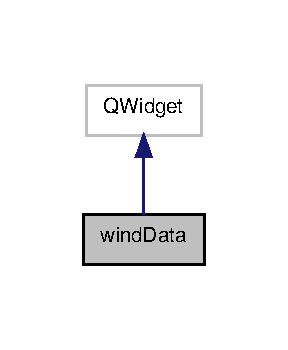
\includegraphics[width=138pt]{classwindData__inherit__graph}
\end{center}
\end{figure}


Collaboration diagram for wind\+Data\+:\nopagebreak
\begin{figure}[H]
\begin{center}
\leavevmode
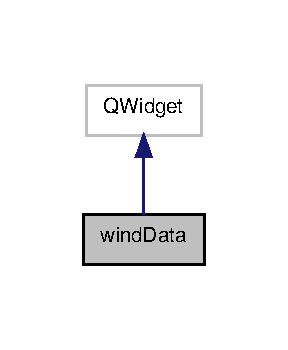
\includegraphics[width=138pt]{classwindData__coll__graph}
\end{center}
\end{figure}
\subsection*{Public Member Functions}
\begin{DoxyCompactItemize}
\item 
\hyperlink{classwindData_a90c7b3022b8bf9a59c35b4d8325be4c7}{wind\+Data} (Q\+Widget $\ast$parent=0)
\end{DoxyCompactItemize}


\subsection{Detailed Description}
Widget to collect wind data and plot a time history on the screen 

\subsection{Constructor \& Destructor Documentation}
\hypertarget{classwindData_a90c7b3022b8bf9a59c35b4d8325be4c7}{\index{wind\+Data@{wind\+Data}!wind\+Data@{wind\+Data}}
\index{wind\+Data@{wind\+Data}!wind\+Data@{wind\+Data}}
\subsubsection[{wind\+Data}]{\setlength{\rightskip}{0pt plus 5cm}wind\+Data\+::wind\+Data (
\begin{DoxyParamCaption}
\item[{Q\+Widget $\ast$}]{parent = {\ttfamily 0}}
\end{DoxyParamCaption}
)}}\label{classwindData_a90c7b3022b8bf9a59c35b4d8325be4c7}


The documentation for this class was generated from the following files\+:\begin{DoxyCompactItemize}
\item 
\hyperlink{windData_8h}{wind\+Data.\+h}\item 
\hyperlink{windData_8cpp}{wind\+Data.\+cpp}\end{DoxyCompactItemize}

\chapter{File Documentation}
\hypertarget{main_8cpp}{\section{main.\+cpp File Reference}
\label{main_8cpp}\index{main.\+cpp@{main.\+cpp}}
}
{\ttfamily \#include $<$Q\+Application$>$}\\*
{\ttfamily \#include \char`\"{}main\+Window.\+h\char`\"{}}\\*
Include dependency graph for main.\+cpp\+:\nopagebreak
\begin{figure}[H]
\begin{center}
\leavevmode
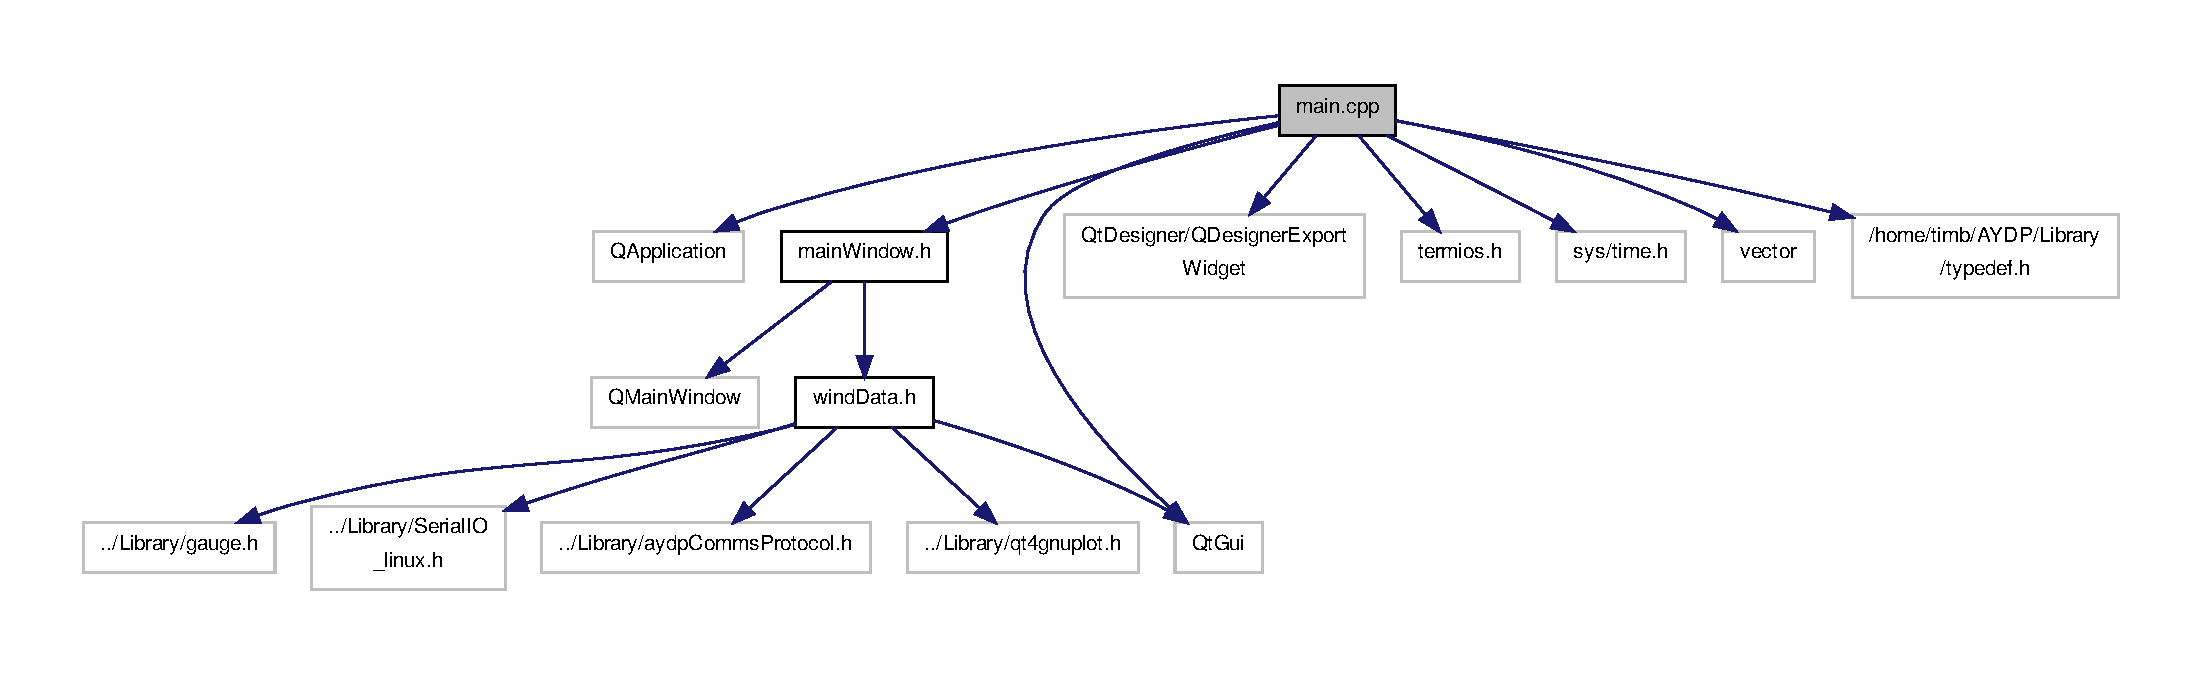
\includegraphics[width=350pt]{main_8cpp__incl}
\end{center}
\end{figure}
\subsection*{Functions}
\begin{DoxyCompactItemize}
\item 
void \hyperlink{main_8cpp_a42662dc47ec6886db83f4fa886f87e32}{header} ()
\item 
int \hyperlink{main_8cpp_a0ddf1224851353fc92bfbff6f499fa97}{main} (int argc, char $\ast$argv\mbox{[}$\,$\mbox{]})
\end{DoxyCompactItemize}


\subsection{Function Documentation}
\hypertarget{main_8cpp_a42662dc47ec6886db83f4fa886f87e32}{\index{main.\+cpp@{main.\+cpp}!header@{header}}
\index{header@{header}!main.\+cpp@{main.\+cpp}}
\subsubsection[{header}]{\setlength{\rightskip}{0pt plus 5cm}void header (
\begin{DoxyParamCaption}
{}
\end{DoxyParamCaption}
)}}\label{main_8cpp_a42662dc47ec6886db83f4fa886f87e32}
\hypertarget{main_8cpp_a0ddf1224851353fc92bfbff6f499fa97}{\index{main.\+cpp@{main.\+cpp}!main@{main}}
\index{main@{main}!main.\+cpp@{main.\+cpp}}
\subsubsection[{main}]{\setlength{\rightskip}{0pt plus 5cm}int main (
\begin{DoxyParamCaption}
\item[{int}]{argc, }
\item[{char $\ast$}]{argv\mbox{[}$\,$\mbox{]}}
\end{DoxyParamCaption}
)}}\label{main_8cpp_a0ddf1224851353fc92bfbff6f499fa97}

\hypertarget{mainWindow_8cpp}{\section{main\+Window.\+cpp File Reference}
\label{mainWindow_8cpp}\index{main\+Window.\+cpp@{main\+Window.\+cpp}}
}
{\ttfamily \#include \char`\"{}main\+Window.\+h\char`\"{}}\\*
Include dependency graph for main\+Window.\+cpp\+:\nopagebreak
\begin{figure}[H]
\begin{center}
\leavevmode
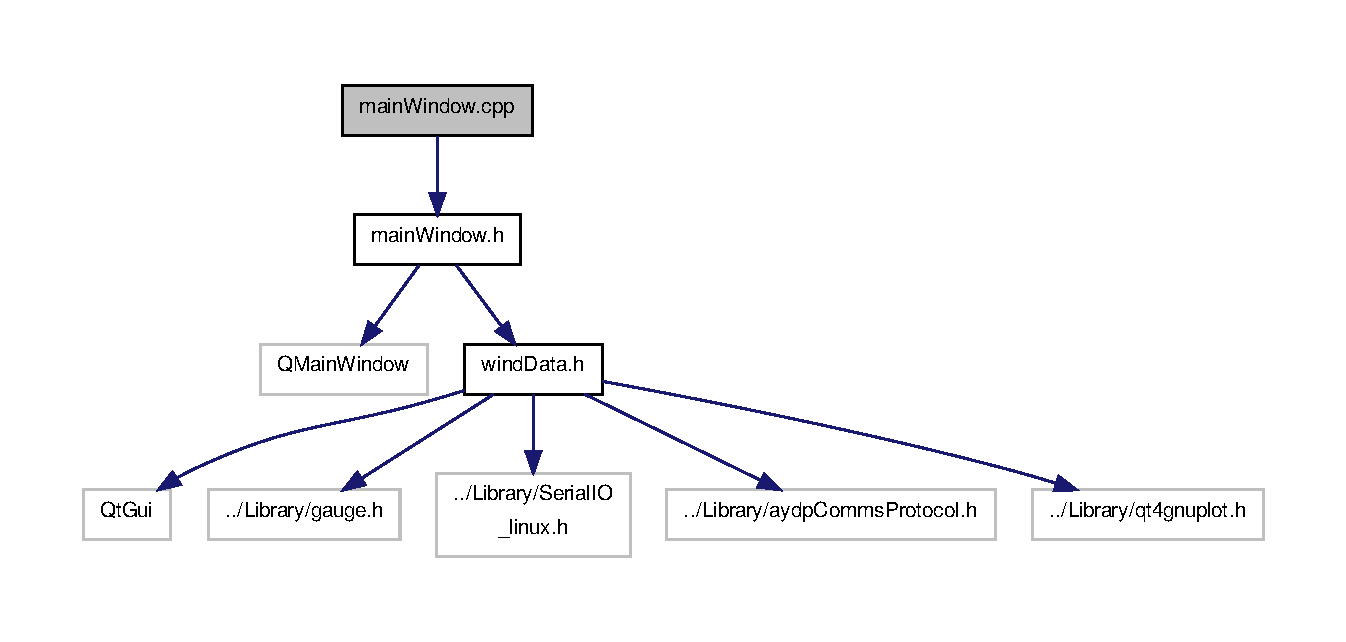
\includegraphics[width=350pt]{mainWindow_8cpp__incl}
\end{center}
\end{figure}

\hypertarget{mainWindow_8h}{\section{main\+Window.\+h File Reference}
\label{mainWindow_8h}\index{main\+Window.\+h@{main\+Window.\+h}}
}
{\ttfamily \#include $<$Q\+Main\+Window$>$}\\*
{\ttfamily \#include \char`\"{}wind\+Data.\+h\char`\"{}}\\*
Include dependency graph for main\+Window.\+h\+:\nopagebreak
\begin{figure}[H]
\begin{center}
\leavevmode
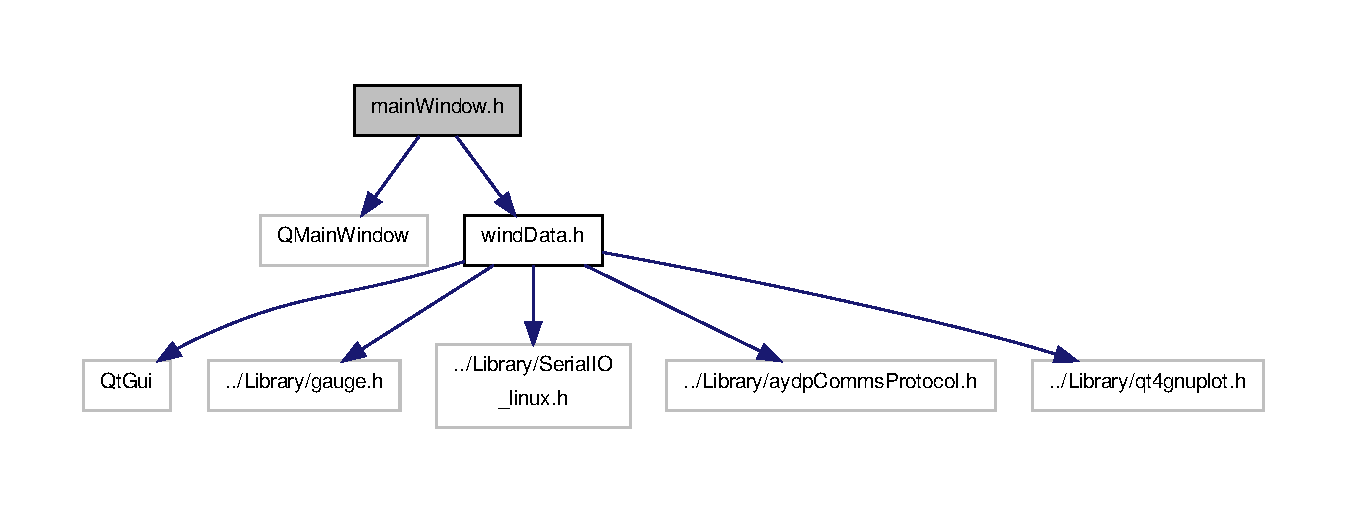
\includegraphics[width=350pt]{mainWindow_8h__incl}
\end{center}
\end{figure}
This graph shows which files directly or indirectly include this file\+:\nopagebreak
\begin{figure}[H]
\begin{center}
\leavevmode
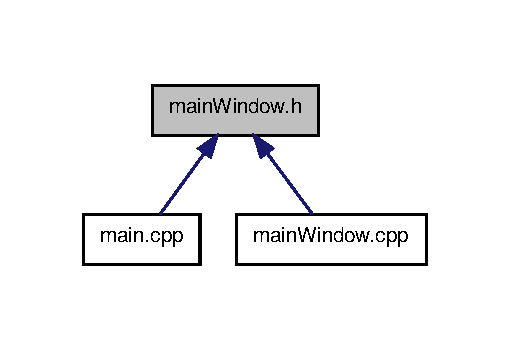
\includegraphics[width=244pt]{mainWindow_8h__dep__incl}
\end{center}
\end{figure}
\subsection*{Classes}
\begin{DoxyCompactItemize}
\item 
class \hyperlink{classmainWindow}{main\+Window}
\end{DoxyCompactItemize}

\hypertarget{windData_8cpp}{\section{wind\+Data.\+cpp File Reference}
\label{windData_8cpp}\index{wind\+Data.\+cpp@{wind\+Data.\+cpp}}
}
{\ttfamily \#include \char`\"{}wind\+Data.\+h\char`\"{}}\\*
{\ttfamily \#include \char`\"{}../\+Library/aydp\+Time.\+h\char`\"{}}\\*
Include dependency graph for wind\+Data.\+cpp\+:\nopagebreak
\begin{figure}[H]
\begin{center}
\leavevmode
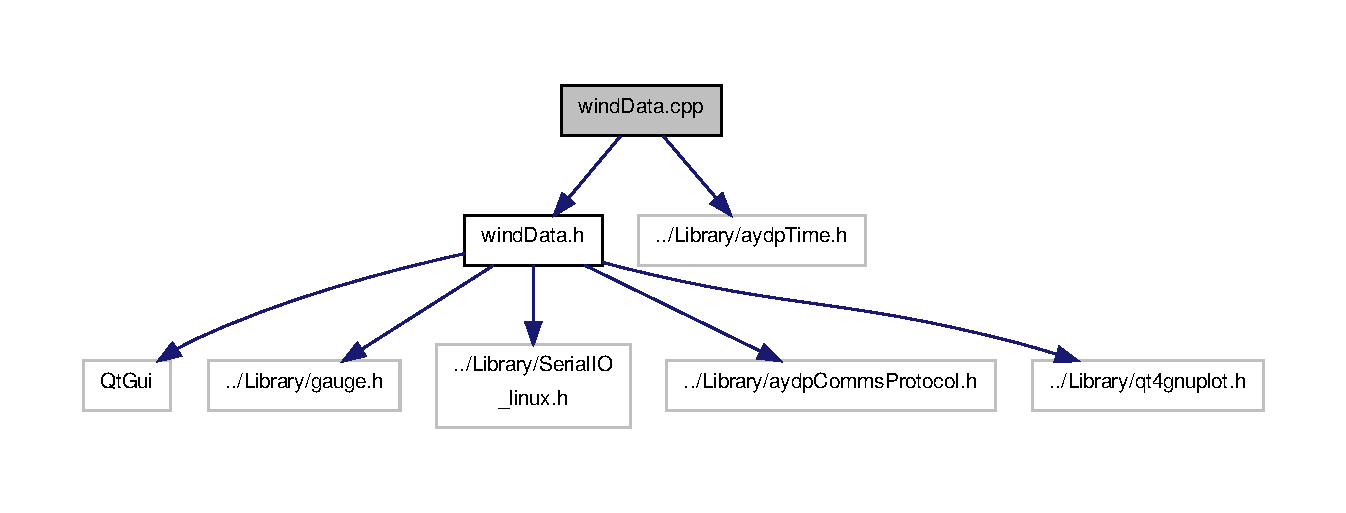
\includegraphics[width=350pt]{windData_8cpp__incl}
\end{center}
\end{figure}

\hypertarget{windData_8h}{\section{wind\+Data.\+h File Reference}
\label{windData_8h}\index{wind\+Data.\+h@{wind\+Data.\+h}}
}
{\ttfamily \#include $<$Qt\+Gui$>$}\\*
{\ttfamily \#include \char`\"{}../\+Library/gauge.\+h\char`\"{}}\\*
{\ttfamily \#include \char`\"{}../\+Library/\+Serial\+I\+O\+\_\+linux.\+h\char`\"{}}\\*
{\ttfamily \#include \char`\"{}../\+Library/aydp\+Comms\+Protocol.\+h\char`\"{}}\\*
{\ttfamily \#include \char`\"{}../\+Library/qt4gnuplot.\+h\char`\"{}}\\*
Include dependency graph for wind\+Data.\+h\+:\nopagebreak
\begin{figure}[H]
\begin{center}
\leavevmode
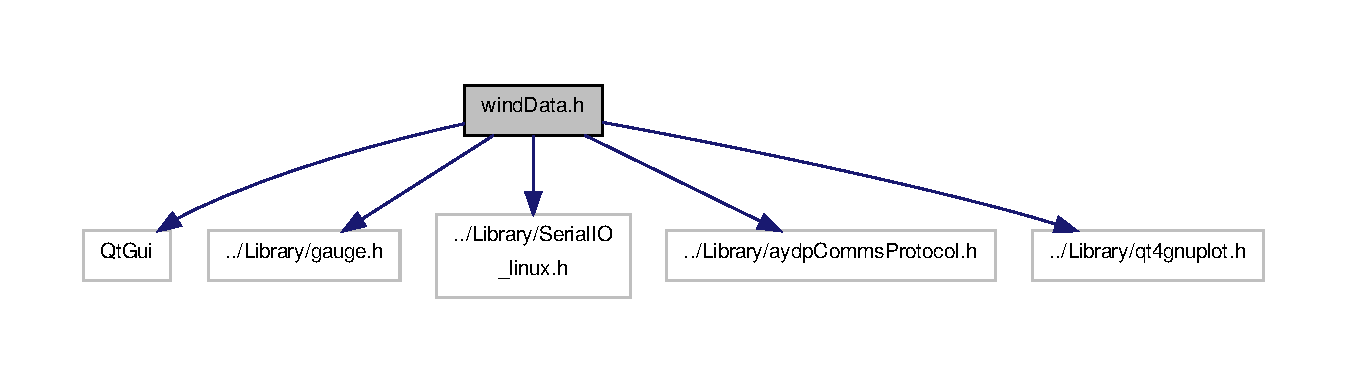
\includegraphics[width=350pt]{windData_8h__incl}
\end{center}
\end{figure}
This graph shows which files directly or indirectly include this file\+:\nopagebreak
\begin{figure}[H]
\begin{center}
\leavevmode
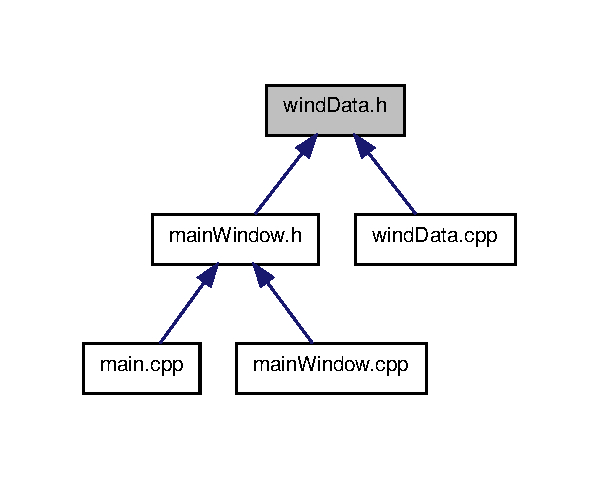
\includegraphics[width=287pt]{windData_8h__dep__incl}
\end{center}
\end{figure}
\subsection*{Classes}
\begin{DoxyCompactItemize}
\item 
class \hyperlink{classwindData}{wind\+Data}
\end{DoxyCompactItemize}

%--- End generated contents ---

% Index
\newpage
\phantomsection
\addcontentsline{toc}{chapter}{Index}
\printindex

\end{document}
